\documentclass[../../DD.tex]{subfiles}
\begin{document}
\section{L-IDM}
	\textit{Musical Instrument} has three dialog acts: the \textit{Description} explains how an instrument works, the \textit{History} is a short explanation about its birth, and the \textit{Image} is a graphic representation of the \textit{Musical Instrument}.
	\textit{Event} and \textit{Course} are represented by similar dialog acts: the \textit{Description}, the \textit{Practical Info}, that contains information about their schedules (specific date for \textit{Event}, periodic days for \textit{Course}), and the \textit{Image}.
	\newline
	\textit{Person} is composed by its \textit{Biography} and an \textit{Image} that is her profile picture. From an \textit{Event} can be useful to check its organizer, to contact her for more information, but the other way around is not important, so there is only one introductory act between \textit{Person} and \textit{Event}.
	\newline
	\textit{Association} topic has a \textit{Description} and an \textit{Image}; \textit{Contacts} topic is composed by \textit{Contacts}, that represents the phone numbers and the email to contact the Association, \textit{Social channels} and \textit{Where we are}, with the address of the office and its map.
	\newline
	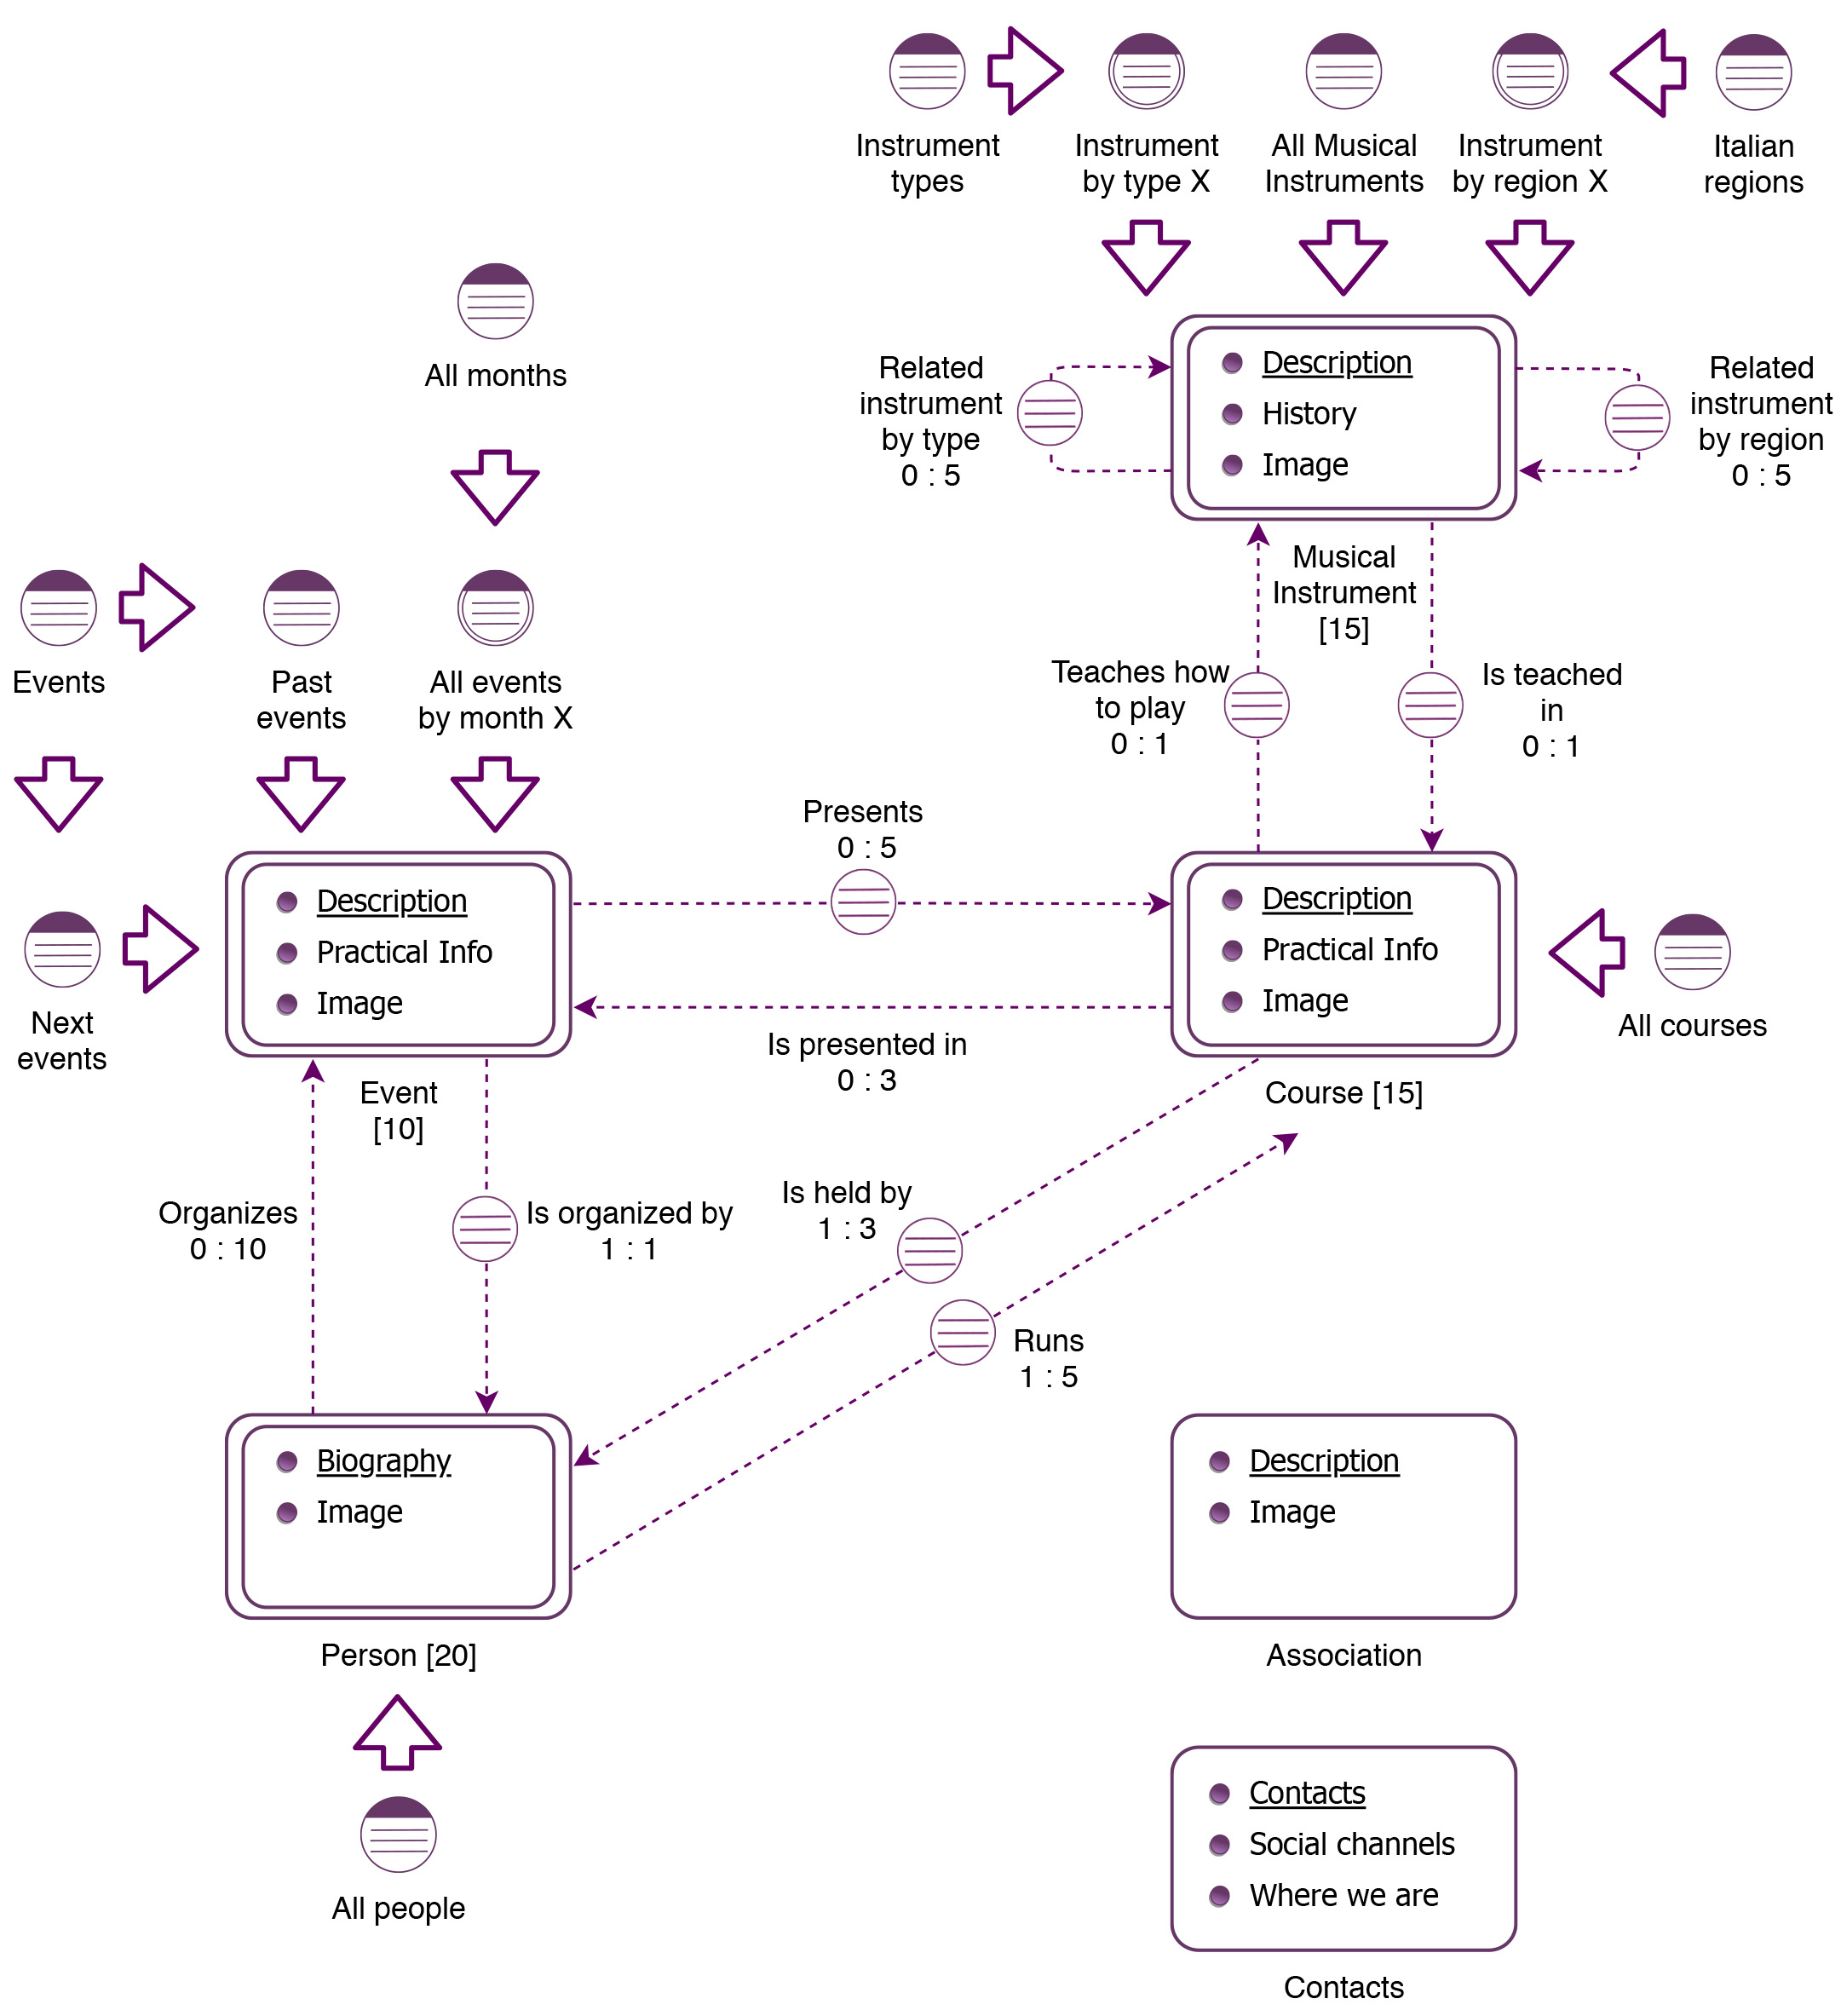
\includegraphics[width=\textwidth,height=\textheight,keepaspectratio]{IDM/L-IDM.jpg}
\end{document}
